%% Digital Systems
%% Digital System Models
\def\FileDate{98/11/18}
\def\FileVersion{1.0}
% ----------------------------------------------------------------
% Notes pages *********************************************************
% ----------------------------------------------------------------

The equivalent of the differential equation model for continuous
systems is the difference equation for digital systems. Replacing
the differential operator $\frac{d}{dt}$ by the advance operator
$\triangle$ gives the general form of the differential equation as
\begin{equation}\label{eq:l9e1}
  \triangle^ny + a_{1}\triangle^{n-1}y + \ldots +  a_n y = b_0
  \triangle^n u + b_{1}\triangle^{n-1} u + \ldots + b_n u.
\end{equation}
Now, given the definition of the advance operator derived in a
previous lecture $$\triangle^n v_k = v_{k+n}$$ we can re-write
equation (\ref{eq:l9e1}) as the \emph{difference equation}
\begin{equation}\label{eq:l9e2}
  y_{k+n} + a_{1}y_{k+n-1} + \ldots + a_n y_k = b_0
   u_{k+n} + b_{1} u_{k+n-1} + \ldots +  b_n u_k.
\end{equation}

Unlike the differential equation, however, which is hardly ever
expressed in an integral form, the difference equation is more
usually expressed in terms of the delay operator $\nabla$.
Applying the operator $\nabla^n$ to equation (\ref{eq:l9e1}) gives
\begin{eqnarray}\label{eq:l9e3}
y + a_{1}\nabla y + \ldots  + a_n \nabla^n y &=& b_0 u +
b_{1}\nabla u + \ldots +  b_n\nabla^n u\\
  y_{k} + a_{1}y_{k-1} + \ldots +  a_n y_{k-n}
   &=& b_0
   u_{k} + b_{1} u + \ldots + b_n u_{k-n}.\label{eq:19e4}
   \end{eqnarray}

Applying the $z$ transform directly to the difference equation
with the delay operator (\ref{eq:l9e3}) gives
\begin{eqnarray}\label{l9e5}
 Y + a_{1}z^{-1} Y + \ldots + a_n z^{-n} Y
&=& b_0 U + b_{1}z^{-1} U + \ldots + b_n z^{-n} U\\ (1 +
a_{1}z^{-1} + \ldots +  a_n z^{-n}) Y &=& (b_0 + b_{1}z^{-1} +
\ldots + b_n z^{-n}) U \label{eq:19e6}
   \end{eqnarray}

\begin{slide}\label{slide:l9s1} \heading{$z$ Transfer Function}
Given that
\[(1 +
a_{1}z^{-1} + \ldots +  a_n z^{-n}) Y(z) = (b_0 + b_1 z^{-1} +
\ldots + b_n z^{-n}) U(z)\] The $z$ transfer function is
\[H(z) = \frac{Y(z)}{U(z)}=\frac{b_0 + b_{1}z^{-1} + \ldots + b_n
z^{-n}}{1 + a_1z^{-1} + \ldots + a_n z^{-n}}\]

A digital system in this general form is known as a
``\emph{pole-zero, infinite impulse response, recursive
auto-regressive moving average digital filter(!)}''
\end{slide}

\begin{slide}\label{slide:l9s2} \heading{$z$ Transfer Function (2)}
If $b_1 = b_2 = \cdots = b_n = 0$ then the transfer function is
\[H(z) = \frac{b_0}{1 + a_1z^{-1} + \ldots + a_n z^{-n}}\]

A digital system in this form is known as an ``\emph{all pole,
infinite impulse response, recursive auto-regressive digital
filter.}''
\end{slide}

\begin{slide}\label{slide:l9s3} \heading{$z$ Transfer Function (3)}
When $a_1 = a_2 = \cdots = a_n = 0$ then the transfer function is
\[H(z) = b_0 + b_{1}z^{-1} + \ldots + b_n
z^{-n}\]

A digital system in this form is known as an ``\emph{all zero,
finite impulse response, non recursive moving average digital
filter.}''
\end{slide}
\begin{slide}\heading{Other forms of digital transfer function}
The transfer function can also be expressed in the
zero-pole-gain form
\[H(z) = \frac{k(z-z_1)(z-z_2)\cdots(z-z_n)}{(z-p_1)(z-p_2)\cdots(z-p_n)}\]
and the partial fraction form
\[H(z) = \frac{r_1}{z-p_1}+\frac{r_2}{z-p_2}\cdots\frac{r_n}{z-p_n}\]
\end{slide}

\begin{slide}\label{slide:l9s4} \heading{Canonical Forms}
\begin{itemize}
\item With the transfer function written as
\[H(z) = \frac{b_0 z^n + b_{n-1} z^{n-1} + \cdots + b_1 z + b_n}{z^n + a_1 z^{n-1} + \cdots + a_{n-1} z + b_n}\]
there is a direct analogy with the general form of the continuous
system transfer function with $s$ instead of $z$. \item That was
implemented with the physically realistic integral operator $\int
dt$ for which the digital equivalent is the delay operator
$\nabla$. \item The operational block diagrams of a digital system
in the various canonical forms is shown in the final sequence of
slides.
\end{itemize}
\end{slide}

\begin{slide}\label{slide:l9s14}
\heading{Controller Canonical Form}
\resizebox{300pt}{!}{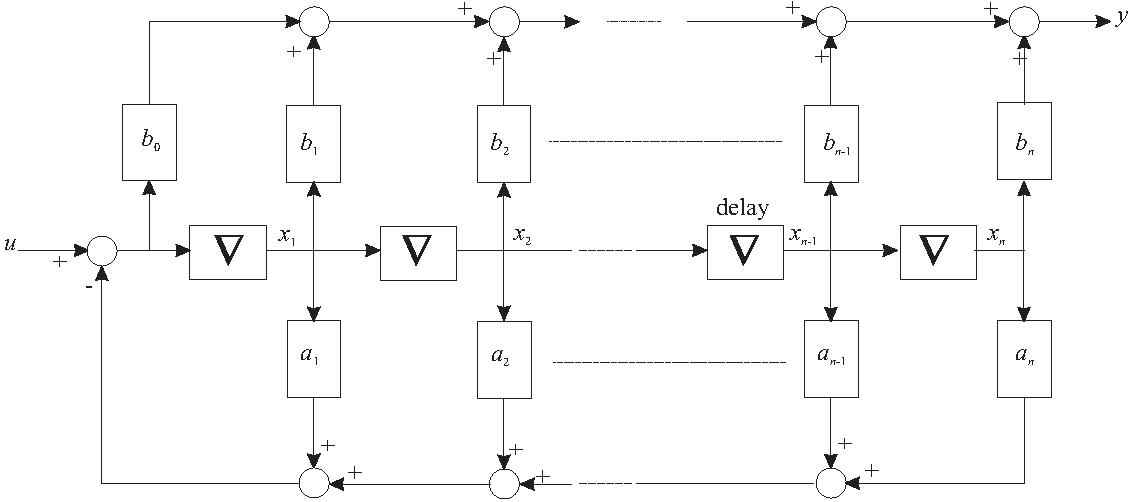
\includegraphics{pictures/dccanon.pdf}}
\end{slide}

\begin{slide}\label{slide:l9s15}
\heading{Observer Canonical Form}
\resizebox{300pt}{!}{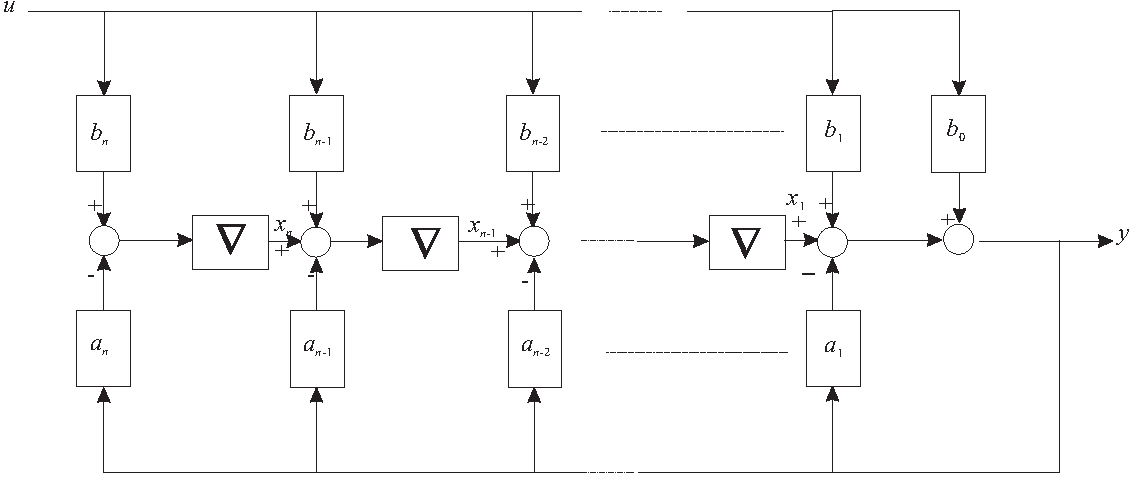
\includegraphics{pictures/docanon.pdf}}
\end{slide}

\begin{slide}\label{slide:l9s16}
\heading{Normal Canonical Form}
\resizebox{300pt}{!}{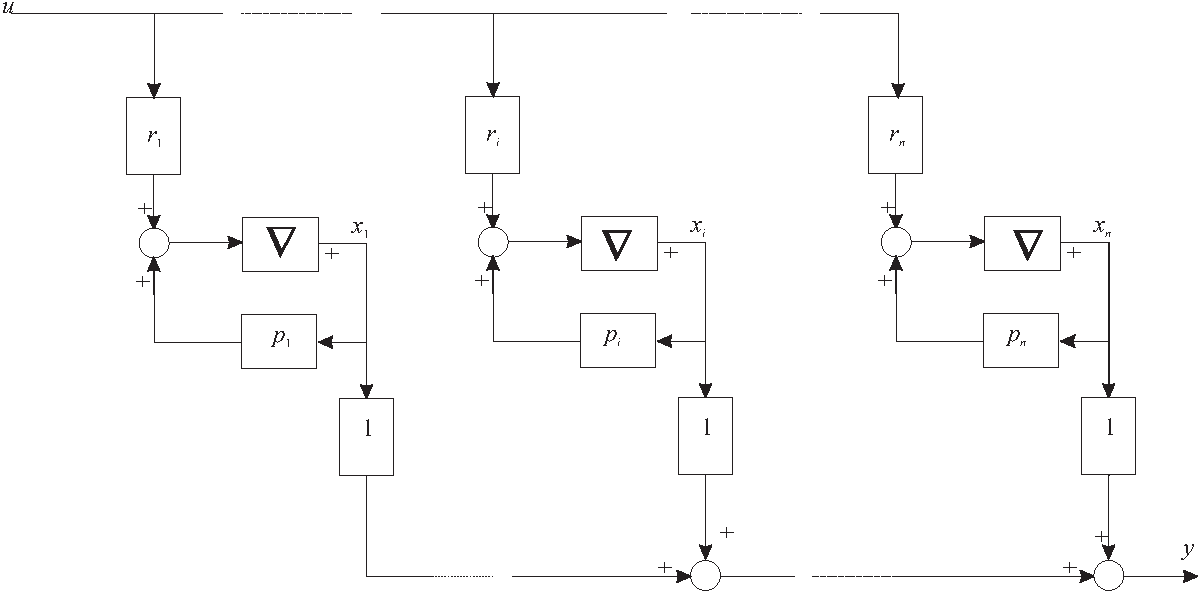
\includegraphics{pictures/dnrmlcan.pdf}}
\end{slide}

In the next lecture we will consider the system response of
systems represented by digital transfer functions.



%----------------------------------------------------------------
% The end of notes
% ----------------------------------------------------------------
\endinput

% Local Variables:
% TeX-master: "lecture8"
% End:
